\documentclass[11pt, addpoints, answers]{exam}

\usepackage{amsmath, amssymb}
\usepackage{xcolor}
\usepackage{tikz}
\usepackage{enumerate}
\usepackage{graphicx}
\usepackage{tabularx}
\usepackage{tikz}
\usepackage{tikz-qtree}
\usetikzlibrary{positioning}
\usetikzlibrary{graphs}
\usetikzlibrary{arrows.meta}

\newcommand{\red}[1]{\textcolor{red}{#1}}
\newcommand{\blue}[1]{\textcolor{blue}{#1}}
% For inserting code snippets.
\usepackage{listings}
\lstset{
    columns = fixed,
    basewidth = {0.5em},
    breaklines = true,
    backgroundcolor = \color{white},
    keywordstyle = \color[RGB]{40, 40, 255},
    numberstyle = \footnotesize\color{darkgray},
    commentstyle = \ttfamily\color{violet},
    basicstyle = \ttfamily,
    stringstyle = \ttfamily\color[RGB]{128, 0, 0},
    showstringspaces = false,
    language = {[11]C++},
    escapechar = \@
}
\lstnewenvironment{cpp}[1][]{\lstset{language = {[11]C++}, #1}}{}

\renewcommand{\baselinestretch}{1.15}
\setlength{\parskip}{1.25\baselineskip}

% headers, footers, titles
\newcommand{\CourseName}{CS101 Algorithms and Data Structures}
\newcommand{\HomeworkNO}{8}
\newcommand{\DueDate}{November 27, 2024}

\pagestyle{headandfoot}
\runningheadrule
\runningheader{CS101 24Fall}{Homework \HomeworkNO}{Due on: \DueDate}
\runningfooter{}{\thepage}{}

\title{
    \vspace{25pt}
    \LARGE ShanghaiTech University \\
    \bigskip
    \textbf{\CourseName} \\
    \textbf{Fall 2024}   \\
    \bigskip
    Homework \HomeworkNO
}
\author{}
\date{Due date: \DueDate, at 23:59}

% formats of questions, choices, points, etc.
\qformat{\bf\thequestion. (\totalpoints\ points) \thequestiontitle\hfill}
\pointname{'}
\SolutionEmphasis{\color{black}}
\CorrectChoiceEmphasis{\bf\color{blue}}



% We frequently use this font.
\newcommand{\ttt}{\texttt}
\newcommand{\bluett}[1]{\textcolor{blue}{\ttt{#1}}}

\begin{document}

\maketitle

\begin{enumerate}
	\item Please write your solutions in English.
	\item Submit your solutions to gradescope.com.
	\item Set your FULL name to your Chinese name and your STUDENT ID correctly in Account Settings.
	\item If you want to submit a handwritten version, scan it clearly. \ttt{CamScanner} is recommended.
	\item When submitting, match your solutions to the problems correctly.
	\item No late submission will be accepted.
	\item Violations to any of the above may result in zero points.
\end{enumerate}

\begin{questions}
	\titledquestion{Multiple Choices}

Each question has \textbf{one or more} correct answer(s). Select all the correct answer(s). For each question, you will get 0 points if you select one or more wrong answers, but you will get 1 point if you select a non-empty subset of the correct answers.

Write your answers in the following table.

%%%%%%%%%%%%%%%%%%%%%%%%%%%%%%%%%%%%%%%%%%%%%%%%%%%%%%%%%%%%%%%%%%%%%%%%%%%
% Note: The `LaTeX' way to answer a multiple-choices question is to replace `\choice'
% with `\CorrectChoice', as what you did in the previous questions. However, there are 
% still many students who would like to handwrite their homework. To make TA's work 
% easier, you have to fill your selected choices in the table below, no matter whether 
% you use LaTeX or not.
%%%%%%%%%%%%%%%%%%%%%%%%%%%%%%%%%%%%%%%%%%%%%%%%%%%%%%%%%%%%%%%%%%%%%%%%%%%

\begin{table}[htbp]
	\centering
	\begin{tabular}{|p{2cm}|p{2cm}|p{2cm}|p{6cm}|}
		\hline
		(a) & (b) & (c) \\
		\hline
		%%%%%%%%%%%%%%%%%%%%%%%%%%%%%%%%%%%%%%%%%%%%%%%%%%%%%%%%%%
		% YOUR ANSWER HERE.
		  BD  &  AC   &  C   \\
		%%%%%%%%%%%%%%%%%%%%%%%%%%%%%%%%%%%%%%%%%%%%%%%%%%%%%%%%%%
		\hline
	\end{tabular}
\end{table}

\begin{parts}
	\part[2] A problem in $\NP$ is $\NPC$ if:
	\begin{choices}
		\choice It can be reduced to another $\NPC$ problem in polynomial time.
		\CorrectChoice There exists a $\NPC$ problem which can be reduced to it in polynomial time.
		\choice It can be reduced to any other $\NP$ problem in polynomial time.
		\CorrectChoice Any other $\NP$ problem can be reduced to it in polynomial time.
	\end{choices}


	\part[2] Assuming that $\P\neq\NP$, which of the following problems are in $\NPC$?
	You may search the Internet for more information if you are unfamiliar with the problems.
	\begin{choices}
		\CorrectChoice \texttt{LONG-PATH}: $(G,s,t,k)$ Given an undirected graph $G$,
		determine whether there exists a simple path from \(s\) to \(t\) whose length is greater or equal to $k$.
		\choice \texttt{HALTING}: $(P,I)$ Given a compilable C++ program $P$ and the input $I$ for $P$,
		determine if $P$ runs infinitely on $I$.
		\CorrectChoice \texttt{4-SAT}: $\phi$ Given a CNF (conjunction normal form)
		where each clause is the disjunction of exactly 4 literals,
		determine whether $\phi$ is satisfiable.
		\choice \texttt{PRIME}: $n$ Given a positive integer $n$, determine whether it is a prime number.
	\end{choices}

	\part[2] For two decision problems $A$ and $B$, suppose that $A\leq_p B$.
	Which of the following statements are true?
	(Hint: there exists complexity classes that are strictly bigger than $\NP$)
	\begin{choices}
		\choice $A\in \P \implies B\in \P$
		\choice $A\in \NPC\implies B\not\in \NPC$.
		\CorrectChoice $B\in \P\implies A\in \P$.
		\choice $B\in \NPC\implies A\in \NPC$.
	\end{choices}

\end{parts}

    \newpage
    \titledquestion{Simulation of MST}
Given a graph $G$ as below: \\
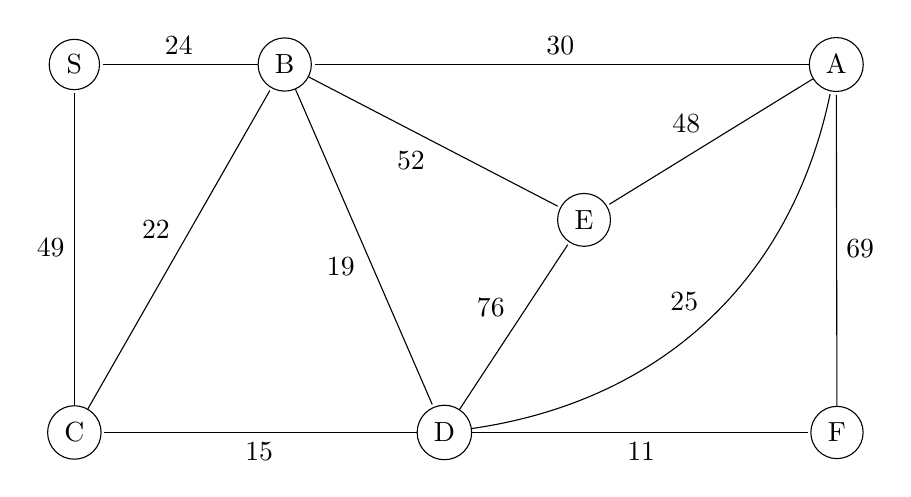
\begin{tikzpicture}[shorten >=1pt,node distance=2cm,auto] 
    \node[circle,draw] (S) {S}; 
    \node[circle,draw] (A) [right=9cm of S] {A}; 
    \node[circle,draw] (B) [right=2cm of S] {B}; 
    \node[circle,draw] (C) [below=4cm of S] {C};
    \node[circle,draw] (D) [right=4cm of C] {D}; 
    \node[circle,draw] (E) [below right=1.5cm and 6cm of S] {E}; 
    \node[circle,draw] (F) [right=9cm of C] {F};
    \path[-] 
    (D) edge [swap] node {11} (F)
    (D) edge [bend right=35] node {25} (A)
    (F) edge [swap] node {69} (A)
    (A) edge [swap] node {48} (E)
    (D) edge node {76} (E)
    (A) edge [swap] node {30} (B)
    (B) edge [swap] node {52} (E)
    (B) edge [swap] node {19} (D)
    (D) edge node {15} (C)
    (C) edge node {22} (B)
    (C) edge node {49} (S)
    (B) edge [swap] node {24} (S);
\end{tikzpicture}
\begin{parts}
    \part[6]
    Use Prim's algorithm to find the Minimal Spanning Tree of the graph. You should select $S$ as the root node. Write the visit order of all nodes. \\
    \textbf{S}$\to$\fillin[][2cm]$\to$\fillin[][2cm]$\to$\fillin[][2cm]$\to$\fillin[][2cm]$\to$\fillin[][2cm]$\to$\fillin[][2cm]
    \part[6] Use Kruskal's algorithm to find the Minimal Spanning Tree of the graph.  Write the edges chosen in order. \\
    \fillin[][2cm]$\to$\fillin[][2cm]$\to$\fillin[][2cm]$\to$\fillin[][2cm]$\to$\fillin[][2cm]$\to$\fillin[][2cm]
    \part[2] Are the MST obtained by Prim's algorithm and the one obtained by Kruskal's algorithm the same? (\textbf{Please write "Yes" or "No".}) 
    \fillin[][2cm]
    
    \part[6] Let's modify the weights of some edges. Please give out the maximum and minimum weight of the edges given that won't change the MST. (You can write $+\infty$ or $-\infty$ if there is no maximum or minimum weight. You should consider every method of breaking ties.)
    \begin{itemize}
        \item AD: 
        Maximum: \fillin[]
        Minimum: \fillin[]
        \item BC:
        Maximum: \fillin[]
        Minimum: \fillin[]
        \item DE:
        Maximum: \fillin[]
        Minimum: \fillin[]
    \end{itemize}
\end{parts}
    \newpage
    \titledquestion{Designing machine}[8]

Fritia is designing a new machine with $n$ components and $m$ wires, with each wires connecting two different components. You can consider this as a connected graph $G=(V, E)$. 
Denote $e_i\in E$ as $e_i = (u_i,v_i,s_i)$ where $e_i$ connects $u_i$-th and $v_i$-th components and has a maximum transmission speed limit $s_i$.

To test her machine, she starts importing data into the $1$st component. Unfortunately, each wire has a distinct maximum transmission speed limit $s_i$. Fritia wants to find a path which can transmit data as fast as possible for each component. \textbf{(The transmission speed limit of a path is the minimum of the maximum transmission speed limit of every wire.)}

Your task is $\forall 2\leq i \leq |V|$, find a path from $1$st component to $i$-th component, which has the fast transmission speed limit. You should give out the steps of your algorithm (\textbf{as efficient as possible}), brief reason of correctness together with the time complexity (tight).

\textbf{Hint:} Recall how Kruskal's works. You can use any algorithm taught in class directly.

\begin{solution}

\end{solution}
    % Very Easy, Even with just 3 tex!
\end{questions}

\end{document}